% to be compiled with xelatex
\documentclass{beamer}
\usepackage{fontspec}
\usepackage[ngerman]{babel}
\usetheme{lankton-keynote}
\begin{document}
\fontspec{Droid Sans}

\title{UniTag 2011: ToureNPlaner}   
\author{} 
\date{16./17. November 2011} 

\frame{\titlepage} 

\frame{\frametitle{Übersicht}\tableofcontents} 

\section{Über uns}
\frame{\frametitle{Wer sind wir?} 
\begin{itemize}
\item 9 Softwaretechnik Studenten
\item 8x Bsc. 5. Semester und 1x Diplom 7. Semester
\item arbeiten gemeinsam dem Studienprojekt ToureNPlaner
\item Leider keine Frauen :(
\end{itemize}
}

\section{Studentenprojekt}
\frame{ \frametitle{Was ein Studienprojekt?}
\begin{itemize}
\item Studienprojekt gehört zum Softwaretechnikstudium
\item Projekt über 2 Semester
    \begin{itemize}
    \item 1 Semester projektspezifische Vorlesung besuchen
    \item 1 Seminar halten
    \item 1. und 2. Semester praktischer Teil (Softwareentwicklung)
    \end{itemize}
\item insgesamt 24 ECTS Punkte (720 Stunden)
\end{itemize}
}

\frame{ \frametitle{Was bringt das Stupro?}
\begin{itemize}
\item {Praxiserfahrung mit „echtem“ Kunden}
\item {Arbeiten in einem großen Team}
\item {Keine Micky Maus Programme}
\item {Programmiererfahrung}
\item {Softskills}
\end{itemize}
}

\frame{ \frametitle{Warum machen wir dieses Projekt?}
\begin{itemize}
\item Interessantes Problem
\item Vielfältige Technologie
\item Netter Kunde
\item Eigene „Besenkammer“
\item ToureNPlaner hat auch noch eine Kaffeemaschine
\end{itemize}
}

\frame{\frametitle{Das Projekt}
ToureNPlaner soll folgende Aufgaben durchführen:
\begin{itemize}
\item {Serveranwendung zur Tourenplanung realisieren}
\item {„Schwere“ Tourenprobleme lösen}
\item {Zugriffsclients realisieren}
\begin{itemize}
\item {Webclient}
\item {Androidclient}
\end{itemize}
\end{itemize}

}
\frame{\frametitle{Motivation}
\begin{itemize}
\item {Nicht triviale Touren berechnen}
\item {Bsp.: Postbote (DHL) will bestmögliche Rundtour finden}
\item {Fahrradrouten mit oberer Grenze an zurückgelegten Höhenmetern finden}
\item Eismann will möglichst viel Gewinn machen
\end{itemize}
}

\frame{\frametitle{Wie macht man sowas?}
Kartenansicht
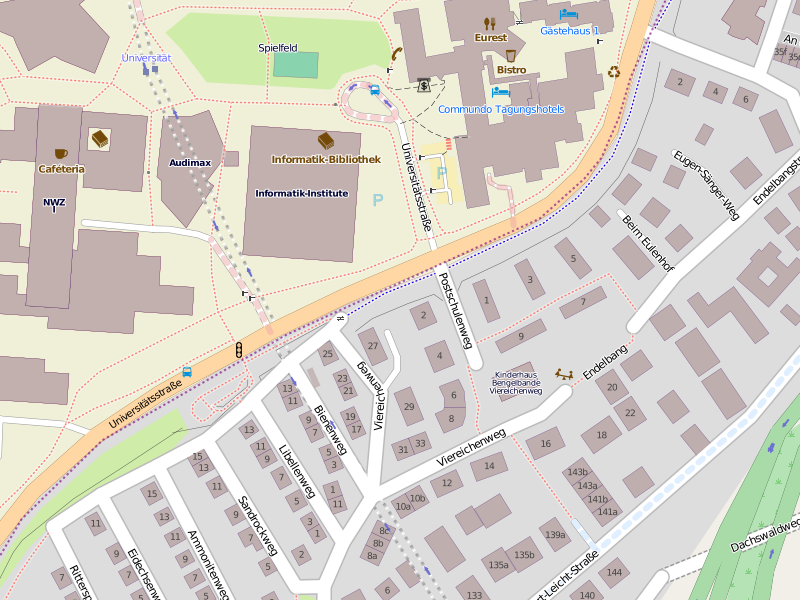
\includegraphics[width =\linewidth]{01.png}}
\frame{\frametitle{Wie macht man sowas?}
Einfügen von Knoten
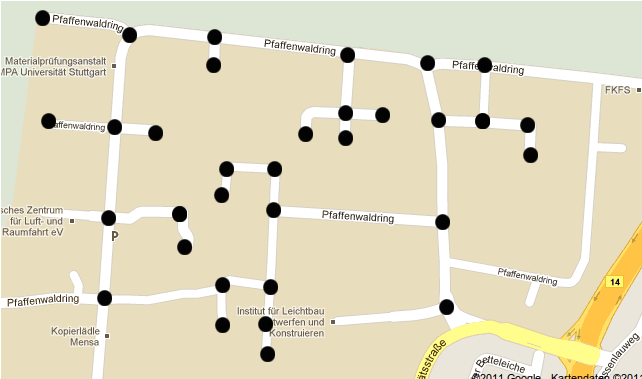
\includegraphics[width =\linewidth]{02.png}}
\frame{\frametitle{Wie macht man sowas?}
Graphen erzeugen
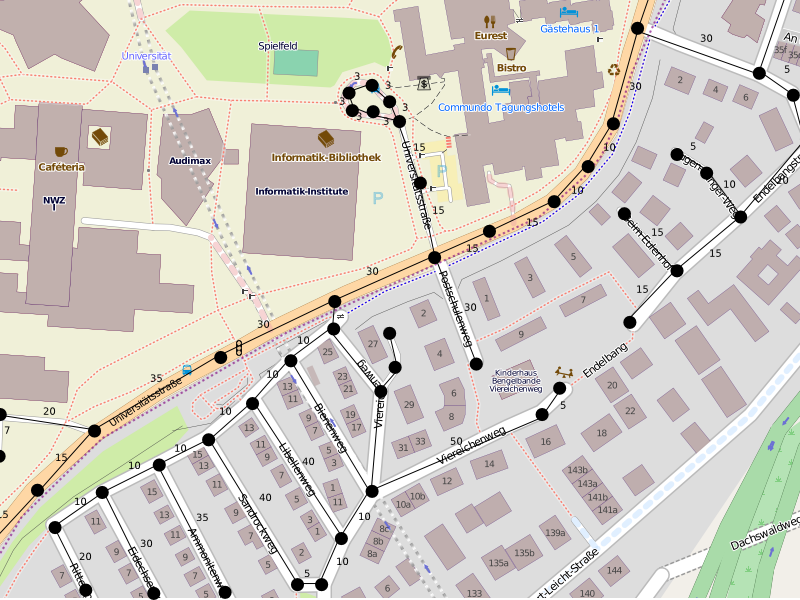
\includegraphics[width =\linewidth]{03.png}}
\frame{\frametitle{Wie macht man sowas?}
Ziel und Startpunkt wählen
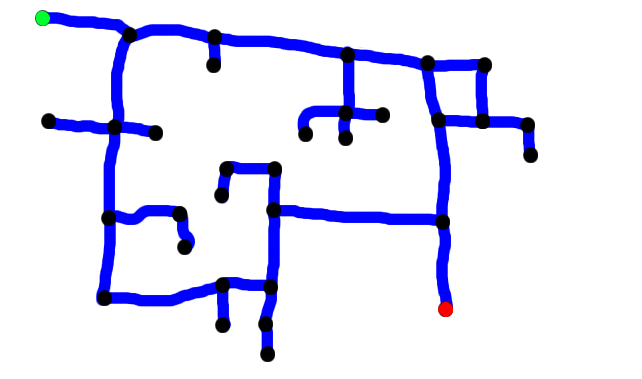
\includegraphics[width =\linewidth]{04.png}}

\section{LiveDemo}
\frame{\frametitle{LiveDemo}
\begin{itemize}
    \item Webclient
    \pause
    \item Android
\end{itemize}
}
\end{document}
